\section{DGSTask Class Reference}
\label{classDGSTask}\index{DGSTask@{DGSTask}}
{\tt \#include $<$DGSTask.h$>$}

Inheritance diagram for DGSTask::\begin{figure}[H]
\begin{center}
\leavevmode
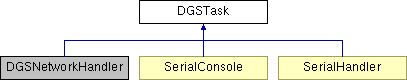
\includegraphics[height=2cm]{classDGSTask}
\end{center}
\end{figure}
\subsection*{Public Member Functions}
\begin{CompactItemize}
\item 
{\bf DGSTask} ()
\item 
virtual int {\bf Is\-Alive} ()
\end{CompactItemize}


\subsection{Detailed Description}
Extents ACE\_\-Task and implements some usefull commands for the Dexterous Grasping System enviroment 



\subsection{Constructor \& Destructor Documentation}
\index{DGSTask@{DGSTask}!DGSTask@{DGSTask}}
\index{DGSTask@{DGSTask}!DGSTask@{DGSTask}}
\subsubsection{\setlength{\rightskip}{0pt plus 5cm}DGSTask::DGSTask ()\hspace{0.3cm}{\tt  [inline]}}\label{classDGSTask_a0}


DGSTask Constructor 

\subsection{Member Function Documentation}
\index{DGSTask@{DGSTask}!IsAlive@{IsAlive}}
\index{IsAlive@{IsAlive}!DGSTask@{DGSTask}}
\subsubsection{\setlength{\rightskip}{0pt plus 5cm}virtual int DGSTask::Is\-Alive ()\hspace{0.3cm}{\tt  [inline, virtual]}}\label{classDGSTask_a1}


Is\-Alive Prints a Message signaling that is alive. As virtual function can be overwrited by descendant classes to personalize their alive messages \begin{Desc}
\item[Returns:]\end{Desc}


Reimplemented in {\bf Serial\-Console} {\rm (p.\,\pageref{classSerialConsole_a4})}.

The documentation for this class was generated from the following file:\begin{CompactItemize}
\item 
{\bf DGSTask.h}\end{CompactItemize}
